%%%%%%%%%%%%%%%%%%%%%%%%%%%%%%%%%%%%%%%%%%%%%%%%%%%%%%%%%%%%%%%%%%%%%%
%\begin{frame}[plain,label=TitlePage]
\begin{frame}[label=TitlePage]
\begin{center}
\textcolor[rgb]{0.2,0.2,0.7}{Structural and electronic instabilities in high pressure CeSb$_2$} \\
\vspace{0.5em}
{\footnotesize Christian de Podesta, c/o Malte Grosche} \\
{\footnotesize \em Cavendish Laboratory, Cambridge} \\
\vspace{0.1em}
\end{center}
\vspace{0.0em}
%\centerline{\multiinclude[<visible@+-| +->][format=pdf,graphics={width=\columnwidth}]{\Figures/FermInstab/QPTScenariosHostGuest2}}
\centerline{ 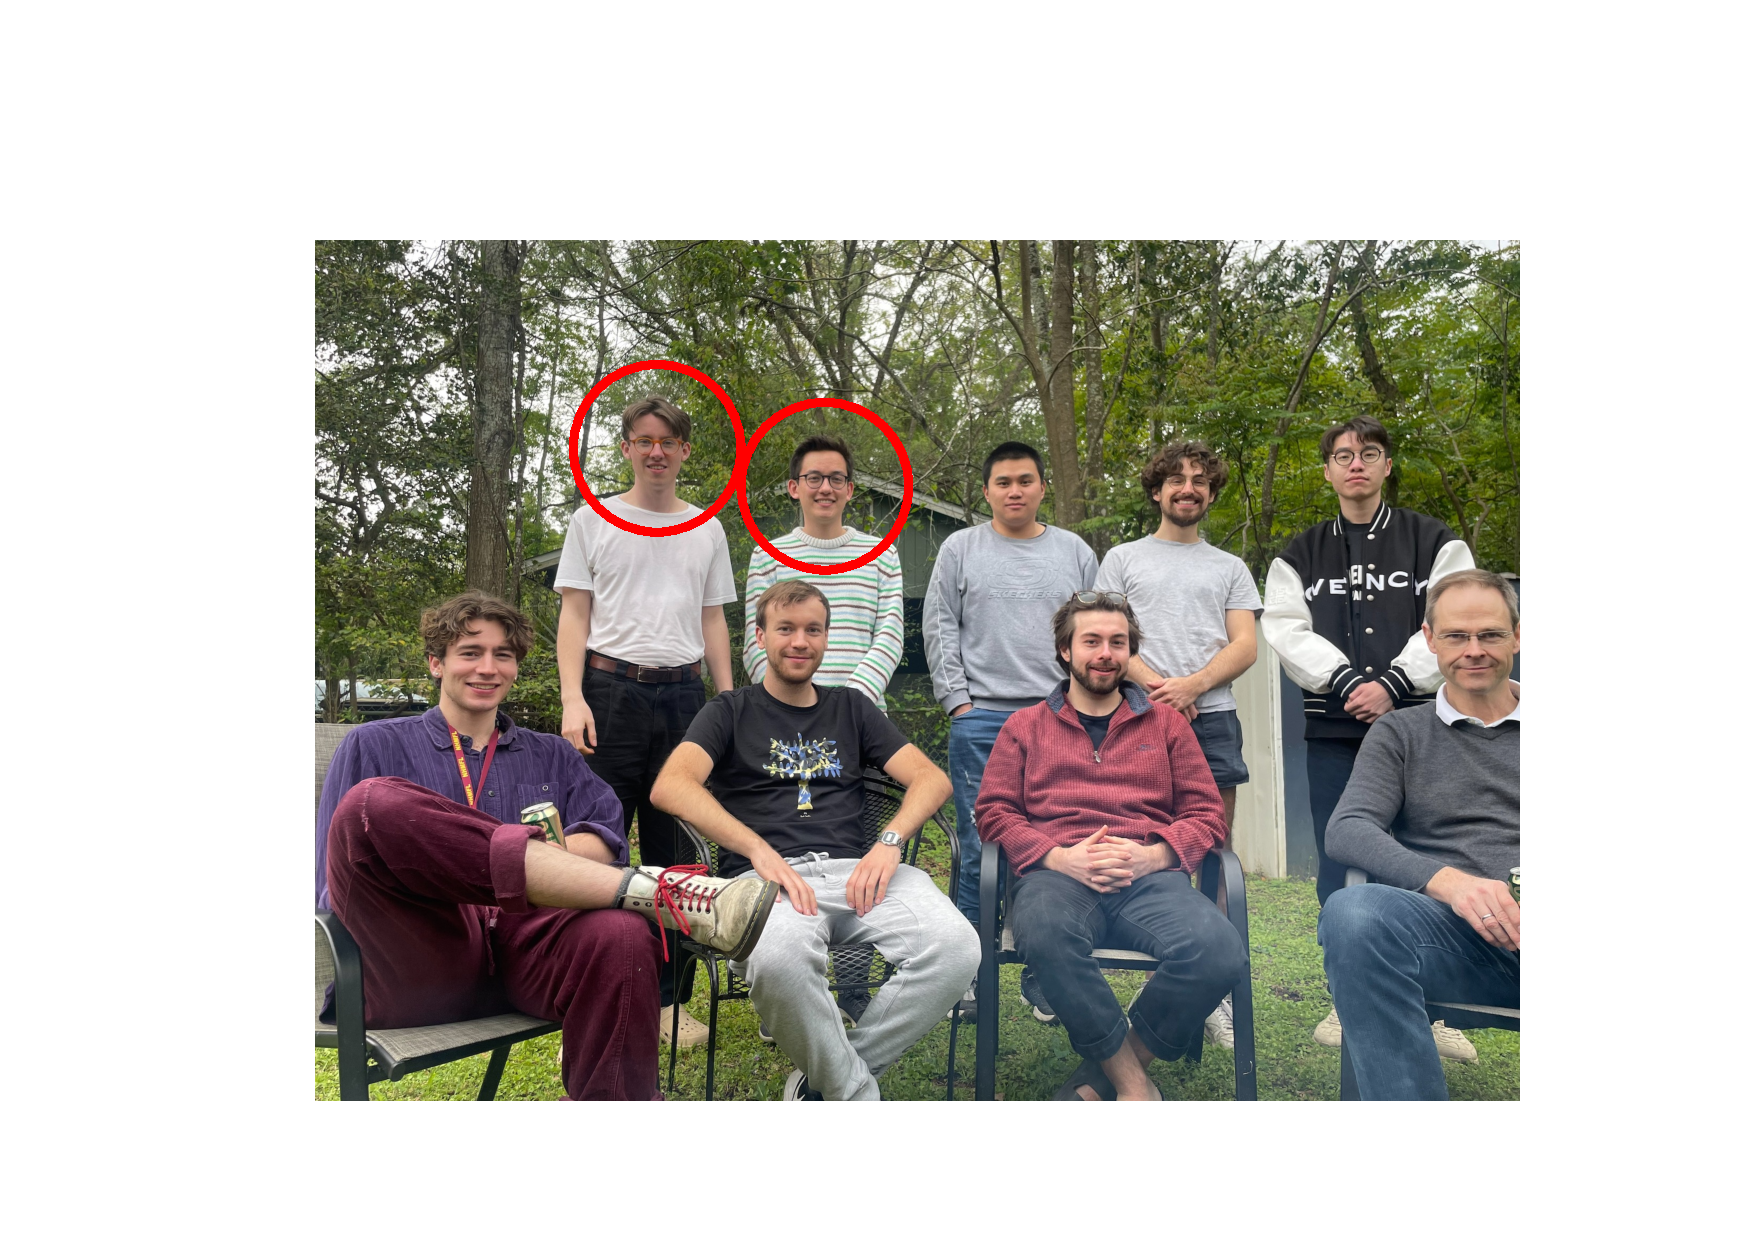
\includegraphics[width=0.75\columnwidth]{GroupPhoto}}

\centerline{\scriptsize The speakers (Christian and Oliver) are still at NHMFL Tallahassee (Cavendish expedition 03/23)}
%\begin{columns}[t]
%\column{0.5\textwidth}
%Narrow electronic bands
%\begin{itemize}
%\item
%Mott transition in NiS$_2$ \\
%{\scriptsize %S. Friedemann {\it et al.} Sci. Rep. {\bf 6,}  416 (2016), \\ 
%Semeniuk  arXiv: 2202.04024 (2022)}
%
%\item
%Mass renormalisation in YFe$_2$Ge$_2$ \\
%{\scriptsize Baglo  Phys. Rev. Lett. {\bf 129,} 046402 (2022)}
%
%\end{itemize}
%
%%\column{0.5 \textwidth}
%Anomalous dissipation
%\begin{itemize}
%\setcounter{enumi}{2}
%\item
%Structural qcp \\
%{\scriptsize L. Klintberg Phys. Rev. Lett. {\bf 109,} 237008 (2012), \\ S. Goh Phys. Rev. Lett. {\bf 114,} 097002 (2015)}
%
%\item
%Quasiperiodic structures \\
%{\scriptsize P. Brown Sci. Adv. {\bf 4:}eaao4793 (2018)}
%\end{itemize}
%
%%\end{columns}
%%
%%\begin{columns}[t]
%%\column{0.25\textwidth}
%%\centerline{~}
%%\column{0.5\textwidth}
%%\centerline{~}
%Both 
%\begin{itemize}
%\setcounter{enumi}{4}
%\item The Kondo lattice system CeSb$_2$
%\end{itemize}
%
%%\end{columns}
%% \visible<4->{
%% \centerline{Quantum degeneracy temperature for electrons in metals: }
%% \[
%% T_F \sim ~\frac{\text{(density)}^{2/3}}{\text{mass}} \simeq 10,000 ~\text{degrees}
%% \]
%% }
%%\begin{itemize}
%%\item
%%Bi-III: incommensurate high pressure structure.
%%
%%% \item Sliding mode $\rightarrow$
%%% strong-coupling superconductivity
%%
%%\item
%%YFe$_2$Ge$_2$: Iron-based superconductor with high $C/T \simeq 100~\text{mJ/molK}^2$.
%%
%%% \item 
%%% New generation of high quality crystals show strong similarity to KFe$_2$As$_2$
%%
%%\end{itemize}
%%
\vspace{0em}
\centerline{\makebox[\linewidth]{\rule{0.85\textwidth}{0.4pt}}}
%\centerline{\scriptsize L. Klintberg Phys. Rev. Lett. {\bf 109,} 237008 (2012), S. Goh Phys. Rev. Lett. {\bf 114,} 097002 (2015)}

\centerline{\scriptsize O. Squire arXiv 2211.00975 (2022)}

\end{frame}

%%%%%%%%%%%%%%%%%%%%%%%%%%%%%%%%%%%%%%%%%%%%%%%%%%%%%%%%%%%%%%%%%%%%%%%
%\begin{frame}[label=QPT]
%\frametitle{Long-range interactions near quantum critical point}
%%\vspace{-3em}
%\centerline{\includegraphics[width=0.9\columnwidth]{\Figures/Phasedias/CePd2Si2/cpsbfaComparison}}
%
%%\vspace{-2em}
%\begin{itemize}
%\item <visible@1-> Long-ranged magnetic correlations near qcp.  %reach to \hl{low energies.}
%
%\item <visible@1-> Mediate pairing interaction, non-Fermi liquid ($\rho \simeq T^{1+\delta}$).
%
%\item <visible@2->  Fine-tuned interaction arising from built-in narrow bands. %Soft modes of the lattice similar?
%
%% \item <visible@6-> High carrier concentration in high-pressure structure.
%\end{itemize}
%
%\vspace*{\fill}
%\centerline{\makebox[\linewidth]{\rule{0.85\textwidth}{0.4pt}}}
%\centerline{\scriptsize Mathur Nature {\bf 394}, 39 (1998), Hashimoto Science {\bf 336,} 1554 (2012))}
%\end{frame}
%
%
%
%
%%%%%%%%%%%%%%%%%%%%%%%%%%%%%%%%%%%%%%%%%%%%%%%%%%%%%%%%%%%%%%%%%%%%%%%
%\begin{frame}[label=LocalMechs]
%\frametitle{Narrow bands via local interactions}
%%\vspace{-3em}
%\begin{columns}[t]
%\column{0.4\textwidth}
%\centerline{~}
%\centerline{\includegraphics[width=\columnwidth]{\data/Figures/Lectures/Mott/MottDOS}}
%\column{0.6\textwidth}
%\centerline{~}
%\begin{itemize}
%\setlength{\itemsep}{1em}
%\item
%Mott: $ U n_{i\uparrow} n_{i\downarrow}$ \\
%$W \rightarrow 0$ at critical $U$
%\item
%Anderson: $ U n_{i\uparrow} n_{i\downarrow} + \text{extra bands}$  \\
%renormalised bands picture
%\item
%Kondo: $J_K S_i s_i $ \\
% $W \sim W_0 \exp({-1/J_K g_0})$
%\item
%Hund's-Kondo: $J'_K \simeq J_K/(2S+1)^2$, $W \sim W_0 \exp({-1/J'_K g_0})$
%\end{itemize}
%\end{columns}
%\end{frame}
%

%%%%%%%%%%%%%%%%%%%%%%%%%%%%%%%%%%%%%%%%%%%%%%%%%%%%%%%%%%%%%%%%%%%%%
% \begin{frame}[plain,label=TitlePage]
% \frametitle{Quantum Matter group}
% \hspace{5em}\includegraphics[width=1.2\columnwidth]{\Figures/GroupAdvertising/GruppenBilder2018}

% \end{frame}







%%% Local Variables: 
%%% mode: latex
%%% TeX-master: "GroTalk.ho"
%%% End: 
